% !TeX root = ../main.tex
% Add the above to each chapter to make compiling the PDF easier in some editors.

\chapter{Background and Related Work}\label{chapter:background}

We explain two research fields that create the bedrock of this thesis, namely, fake news detection and
explainable artificial intelligence. Both areas provide the foundation of tools used in this work. The first
provides the mechanisms and approaches to detect fake news, and the second offers a suite of techniques to interpret these mechanisms and strategies.\\
Initially, in \ref{sec:fakeNewsDetection}, we discuss societal challenges, the characteristics, and the history of fake news. Then we talk about the detection methods that were developed over the years. After showing the challenges of creating FND models, we conclude the first section with SOTA FND models.\\
After fake news detection, in \ref{sec:explainableArtificialIntelligence}, we first examine when XAI is necessary and its importance. Then, we define the suite of explainable artificial intelligence and the goals of XAI, and finally, we determine the suite that aims to satisfy these goals.\\
\section{Fake News Detection}
\label{sec:fakeNewsDetection}
In the past decade, social media has become a place where anyone can share information. Although fast, free, and easy to access, obtaining real news from social media can be difficult, and one should do so at their own risk and always check the facts~\parencite{SocialMediaAndFakeNewsIn2016Election_Allcott,TheScienceOfFakeNews_Lazer}. Nevertheless, the news stream never ends; thus, the need to verify the credibility of news using automated systems arises. To address this necessity, the number of studies involving \emph{Fake News} or \emph{Fake News Detection} has dramatically increased in the last decade (Fig. \ref{fig:FN_vs_FND_Publications}).
\begin{figure}
    \centering
    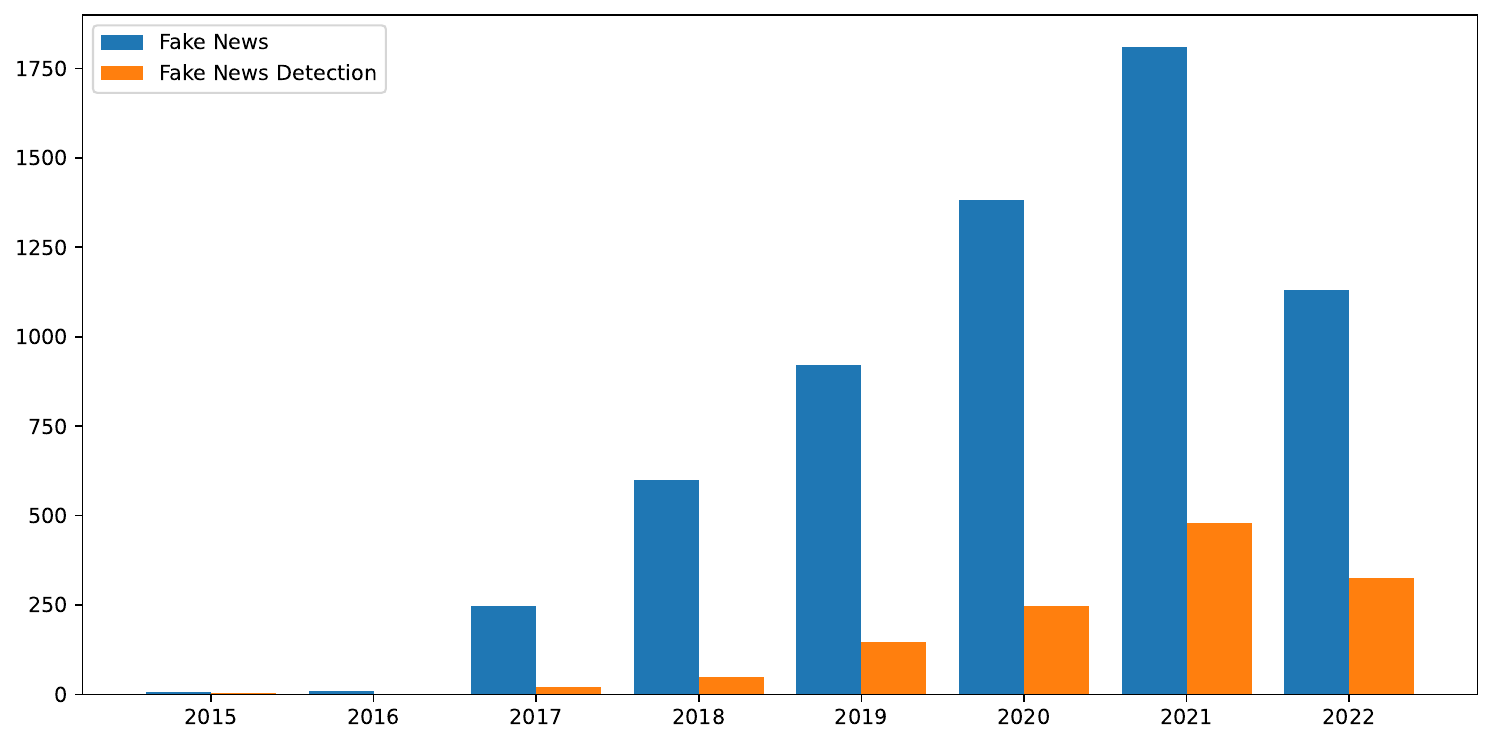
\includegraphics[scale=0.5]{FN_vs_FND_Publications}
    \caption[Fake News and Fake News Detection Publications by Year]{Total number of publications that include (1) \emph{Fake News} (blue) and (2) \emph{Fake News Detection} (orange) publications by year. Source: Scopus; Search Arguments: (1) TITLE-ABS-KEY("fake news*") PUBYEAR AFT 2014 (2) TITLE-ABS-KEY("fake news detection")}\label{fig:FN_vs_FND_Publications}
\end{figure}\\
In \ref{subsec:fakeNewsDetection_fakeNews}, we briefly present the history of fake news and look at studies that display the impact of fake news on society. In this section, we also define the terms fake news, disinformation, and misinformation. \\
In \ref{subsec:fakeNewsDetection_FoundationsOfFakeNews}, we make an excursion into social sciences and human psychology, delivering insights into why humans fall for or tend to believe fake news. Furthermore, we draw some insights from the social, technical, and data-oriented foundations of fake news.\\
We then list the available datasets used in FND and deliberate their advantages and disadvantages in \ref{subsec:fakeNewsDetection_Evolution}. Finally, in \ref{subsec:fakeNewsDetection_Evolution}, we summarize the evolution of detection algorithms, then we classify FND algorithms with respect to their input data type and what they focus on that data.

\subsection{Fake News}
\label{subsec:fakeNewsDetection_fakeNews}
Throughout history, various forms of widespread fake news have been recorded. For instance, in the thirteenth
century BC, Rameses the Great decorated his temples with paintings that tell stories of victory in the Battle
of Kadesh. However, the treaty between the two sides reveals that the battle's outcome was a
stalemate~\parencite{HistorysGreatestLies_Weir}. Just after the printing press was invented in 1439, the
circulation of fake news began. One of history's most famous examples of fake news is the
“Great Moon Hoax”~\parencite{TheGreatMoonHoax_Foster}. In 1835, The Sun newspaper of New York published articles about a real-life astronomer and a made-up colleague who had observed life on the moon. It turns out that these fictionalized articles brought them new customers and almost no backlash after the newspaper admitted that the articles mentioned earlier were a hoax\footnote{https://www.politico.com/magazine/story/2016/12/fake-news-history-long-violent-214535/}.\\
In order to highlight the difference, using the definitions from~\parencite{ThePsycologyOfFakeNews_Pennycook}, we formally introduce the terms disinformation and misinformation as follows.
\begin{definition}[\emph{Disinformation}]
    "\emph{Information that is false or inaccurate and was created with a deliberate intention to mislead people.}"~\parencite{ThePsycologyOfFakeNews_Pennycook}
\end{definition}
\begin{definition}[\emph{Misinformation}]
    "\emph{Information that is false, inaccurate, or misleading. Unlike disinformation, misinformation does not necessarily need to be created deliberately to mislead.}"~\parencite{ThePsycologyOfFakeNews_Pennycook}
\end{definition}
There is no fixed definition for fake news. Thus, we elaborate on the definitions of fake news. A limited definition is news articles that are intentionally or verifiably false~\parencite{SocialMediaAndFakeNewsIn2016Election_Allcott}. This definition stresses authenticity and intent. The inclusion of false information that can be confirmed refers to authenticity. On the other hand, intent refers to the deceitful intention to delude news consumers~\parencite{FakeNewsDetectionOnSocialMediaADataMiningPerspective_Shu}. This definition is widely used in other studies~\parencite{AutomaticDeceptionDetection_Conroy, TheFakeNewsSpreadingPlague_Mustafaraj, FakeNewsDetectionOnSocialMediaADataMiningPerspective_Shu}.\\
Furthermore, recent social sciences studies~\parencite{TheScienceOfFakeNews_Lazer, ThePsycologyOfFakeNews_Pennycook} define fake news as fabricated information that mimics news media content in form but not in organizational process or intent. Similarly, this definition covers authenticity and intent; additionally, it includes the organizational process. More general definitions for fake news consider satire news as fake news due to the inclusion of false information even though satire news aim to entertain and inherently reveals its deception to the consumer~\parencite{WhenFakeNewsBecomesReal_Balmas, TheImpactOfRealNewsAboutFakeNews_Brewer, NewsVerificationByExploitingConflictingSocialViewpoints_Jin, FakeNewsOrTruthUsingSatiricalCues_Rubin}. Further definitions include hoaxes, satires, and obvious
fabrications~\parencite{DeceptionDetectionForFakeNews3TypesOfFakeNews_Rubin}
In this thesis, we are not interested in the organizational process and do not consider conspiracy theories~\parencite{ConspiracyTheories_Sunstein}, superstitions~\parencite{Superstition_Lindeman}, rumors~\parencite{RumorsAndHealthCareReform_Berinsky}, misinformation, satire, or hoaxes. Therefore, we use the limited definition from~\parencite{SocialMediaAndFakeNewsIn2016Election_Allcott} and formally introduce it.
\begin{definition}[\emph{Fake News}]
    "\emph{News articles that are intentionally or verifiably false.}"~\parencite{SocialMediaAndFakeNewsIn2016Election_Allcott}
\end{definition}
Fake news can lead to disastrous situations, such as crashes in stock markets, resulting in millions of dollars. For example, Dow Jones
industrial average went down like a bullet (see Fig. \ref{fig:MarketReactionToFakeTweet}) after a tweet about an explosion injuring President Obama
went out due to a hack~\parencite{MarketQuaversAfterFakeAPTweet_ElBoghdady}.
\begin{figure}
    \centering
    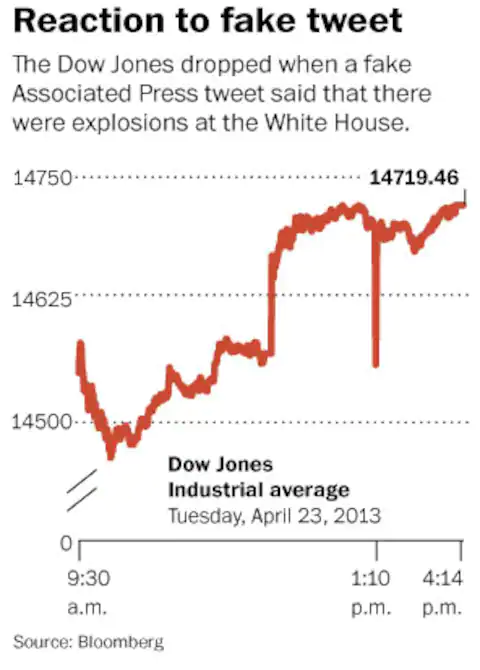
\includegraphics[scale=0.2]{MarketReactionToFakeTweet}
    \caption[Market Reaction to Fake Tweet]{The market's reaction to the fake tweet. The sharp decline caused by a single tweet. Image obtained from~\parencite{MarketQuaversAfterFakeAPTweet_ElBoghdady}}\label{fig:MarketReactionToFakeTweet}
\end{figure}\\
The detrimental impacts of fake news further extend to societal issues.
When fake news rose to prominence with the 2016 U.S. Presidential Election~\parencite{USPresidentialElection2016}, a man, convinced by what he
read on social media about a pizzeria trafficking humans, went on a shooting spree in that pizzeria. Later named
Pizzagate~\parencite{Pizzagate_Fisher}, this incident illustrates the deadly impact of fake news. In fact, fake news can even affect presidential elections~\parencite{SocialMediaAndFakeNewsIn2016Election_Allcott, TrumpWonBecauseOfFacebook_Read}.\\
Recent history exhibits that some fake news spreads like wildfires through social media. Evidence shows that the most popular fake news stories
were more widely shared than the most popular mainstream news stories~\parencite{Buzzfeed_FakeNewsOutperformRealNews_Silverman}.\\
Digital News Report 2022~\parencite{ReutersInstituteDigitalNewsReport} reports in its key findings that trust in the news is 42\% globally,
the highest (69\%) in Finland, and the lowest (26\%) in the U.S.A. Additionally, the same study shows that in early 2022, in the week of the
survey, between 45\% and 55\% of the surveyed social media consumers worldwide witnessed false or misleading information about COVID-19. The
same study also reports the appearance of fake news in politics was between 34\% and 51\%, and between 9\% and 48\% for fake news about
celebrities, global warming, and immigration~\parencite{StatistaUsageOfSocialMedia_Watson}.
\begin{figure}
    \centering
    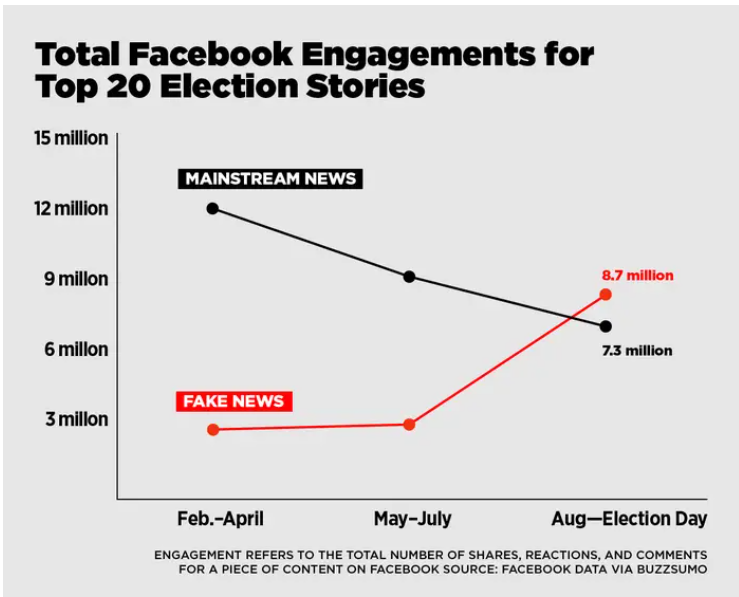
\includegraphics[scale=0.4]{TotalFacebookEngagementsForTop20ElectionStories}
    \caption[Total Facebook Engagements for Top 20 Election Stories]{The rising engagement for fake news stories observed after May-July, just before Presidential Elections. Image obtained from~\parencite{Buzzfeed_FakeNewsOutperformRealNews_Silverman}}\label{fig:TotalFacebookEngagementsForTop20ElectionStories}
\end{figure}
\subsection{Foundations of Fake News}
\label{subsec:fakeNewsDetection_FoundationsOfFakeNews}
The environment for fake news has been the traditional news media for a long time. First started with newsprint,
then continued with radio and television, and now with social media and the web, the dissemination of fake news reached its peak. Next, we discuss the psychological and social foundations of fake news to stress the importance
of human psychology, especially when accepting fake news as genuine and sharing it with others. Then we focus on
the technical foundations where we discuss how social media and technologiy have accelerated the diffusion of fake news.\\
\textbf{Psychological Foundations.}  Understanding the difference between real and fake news is not an easy task
for a human. Two psychological theories, namely, \emph{naive realism} and \emph{confirmation bias}, examine why humans fall for fake news. The first refers to a person's disposition to believe that their point of view is the
mere accurate one, while people who believe otherwise are uninformed or biased~\parencite{NaiveRealism_Reed}.
The second, often called selective exposure, is the proclivity to prefer information that confirms existing views~\parencite{ConfirmationBias_Nickerson}.\\
Another reason for human fallacy in fake news is that once a misperception is formed, it becomes difficult to correct. In fact, it turns out that correcting people leads them to believe false information more, especially
when given factual information that refutes their beliefs~\parencite{WhenCorrectionsFail_Nyhan}.\\
\textbf{Social Foundations.}  The prospect theory explains the human decision-making process as a mechanism
based on maximizing relative gains and minimizing losses with respect to the current
state~\parencite{ProspectTheory_Kahneman, AdvancesInProspectTheory_Kahneman}. This inherent inclination to get the highest reward also applies to social cases in which a person will seek social networks that provide them with
social acceptance. Consequently,  people with different views tend to form separate groups, which makes them feel safer, leading to the consumption and dissemination of information that agrees with their opinions. These behaviors are explained by social identity theory~\parencite{SocialIdentityTheory_Ashforth} and normative social influence~\parencite{NormativeSocialInfluence_Asch}.\\
Two psychological factors play a crucial role here~\parencite{TheRussianFirehoseOfFalsehood_Paul}. The first, social credibility, is explained by a person’s tendency to recognize a source as credible when that source is deemed credible by other people. The second, called the frequency heuristic, is the acceptance of a news piece by repetitively being exposed to it. Collectively, these psychological phenomena are closely related to the well-known filter bubble~\parencite{TheFilterBubble_Pariser}, also called echo chamber, which is the formation of homogenous bubbles in which the users are people of similar ideologies and share similar ideas. Being isolated from different views, these users usually are inclined to have highly polarized opinions~\parencite{EchoChambers_Sunstein}. As a result, the main reason for misinformation dispersal turned out to be the echo
chambers~\parencite{TheSpreadingOfMisinformationOnline_DelVicario}.\\
\textbf{Technical Foundations.} Social media's easy-to-use and connected nature give rise to more people selecting or even creating their own news source. Naturally, this gives way to more junk information echoing in a group of people on social media. As algorithms evolve to understand user preferences, social media platforms recommend similar people or groups to those in echo chambers. A recent study~\parencite{TheEffectOfPeopleRecommenderOnEchoChambers_Cinus}  shows that these recommenders can strengthen these echo chambers. They discuss that some of these recommenders contribute to the polarization on social media. In other words, people can convince themselves that any fake news is real by staying in their echo chambers. One main reason that some fake news spreads so rapidly on social media is the existence of malicious accounts. The account user can be an actual human or a social bot since creating accounts on social media is no cost and almost no effort. While many social bots provide valuable services, some were designed to harm, mislead, exploit, and manipulate social media discourse. Formally, a social bot is a social media account governed by an algorithm to fabricate content and interact with other users~\parencite{TheRiseOfSocialBots_Ferrara}. A more recent study from the same author shows that malicious social bots were heavily used in the 2016 U.S. Presidential Elections~\parencite{SocialBotsDistortThe2016USPresidentialElection_Bessi}. On the other hand, malicious accounts that are not bots, such as online trolls who aim to trigger negative emotions and humans that provoke people on social media to get an emotional response, contribute to the proliferation of fake news~\parencite{AnyoneCanBecomeATroll_Cheng}.\\
Building upon three foundations, we draw some results for fake news to be considered when building a fake news detection model:
\begin{enumerate}
    \item \emph{Invasive}: Fake news can appear on anyone’s feed if it spreads for a sufficient amount of time.
    \item \emph{Hard to discern}: Fake news is fabricated in such a way that it resembles the authenticity of a real news source. This
          indistinguishability leads to issues when working with news-content-based FND models.
    \item \emph{The source is crucial}: The credibility of a news source is essential. We can use news from credible sources to teach the model
          to distinguish genuine from fabricated.
    \item \emph{Fake news has hot spots}: The echo chambers are invaluable examples when trying to understand the behaviors of fake news. We can
          leverage this attribute and use social models, such as graphs, to successfully detect fake news.
    \item \emph{Early detection is essential}: As discussed in psychological foundations, the volume of exposure to a piece of fake news can significantly affect one’s opinions, thus leading to more misinformed individuals.
\end{enumerate}
\textbf{Data-Oriented Foundations.} We define features for news content and social context to represent the news pieces in a structured manner. First, we introduce attributes for news content~\parencite{FakeNewsDetectionOnSocialMediaADataMiningPerspective_Shu}:
\begin{itemize}
    \item \emph{Source}: Publisher of the news piece.
    \item \emph{Headline}: Short title text that aims to catch the readers’ attention and describes the article's main topic.
    \item \emph{Body Text}: The main text piece that details the news story.
    \item \emph{Image/Video}: Part of the body content supplies visual input to articulate the story.
\end{itemize}
Using these attributes, we extract two types of features for news content:
\begin{description}
    \item{\emph{Linguistic-based features}:} The news content is heavily based on textual content. Thus, the first feature that belongs to this class is lexical features which make use of character and word level frequency information which can be obtained by the utilization of
    \emph{term frequency}-\emph{inverse term frequency} (TF-IDF)~\parencite{TF_Luhn, IDF_Jones}. The second feature is based on syntactic features which include sentence-level features that can be obtained via n-grams and bag-of-words (BoW) and punctuation and parts-of-speech (POS)~\parencite{POS_Daelemans} tagging. We can extend these features to domain-specific ones, such as external links and the number of graphs~\parencite{AStylometricInquiry_Potthast}.
    \item{\emph{Visual-based features}:} Particularly for fake news, the visual content is a strong tool for establishing
    belief~\parencite{VisualMisAndDisinformation_Viorela}. Hence, the features that reside in images and videos become significant. Fake images
    and videos which brings the fake story together are commonly used(e.g.~\cite{PutinBehindBars_Harding, DeepFakeQueensSpeech_Sawer}). To counteract the effects of misleading visual input, recent studies~\parencite{ExploitingMultiDomainVisualInformation_Qi} examined visual and statistical information for fake news detection. Visual features consist of clarity score, similarity distribution histogram, diversity score, and clustering score. Statistical features are listed
    as count, image ratio, multi-image ratio etc.~\parencite{FakeNewsDetectionOnSocialMediaADataMiningPerspective_Shu}.
\end{description}
Now, we define features for social context, which has recently drawn much attention from the research community~\parencite{BeyondNewsContents_Shu, HierarchicalPropagationNetworksForFND_Shu}. Overall, we will concern three aspects of social context data: user-based, post-based, and network-based features.
\begin{description}
    \item{\emph{User-based}:} As mentioned in the Technical Foundations part of this subsection, fake news has various ways of disseminating, such as via echo chambers, malicious accounts, or bots. Therefore, analyzing user-based information can prove useful. We distinguish user-based features at the group and individual levels~\parencite{FakeNewsDetectionOnSocialMediaADataMiningPerspective_Shu}. Individual levels are extracted to deduce the credibility of each user by utilizing, for example, the number of followers and followees, the number of tweets authored by a user, etc~\parencite{InformationCredibilityOnTwiter_Castillo}. On the other hand, group-level user-based features are the general characteristics of groups of users related to the news~\parencite{AutomaticDetectionOfRumor_Yang}. Parallel to the social identity theory and normative social influence idea, the assumption is the consumers of real and fake news tend to form different groups, which may lead to unique characteristics. Typical group-level features stem from individual-level features by obtaining the share of verified users, and the average number of followers and followees~\parencite{DetectRumorsUsingTimeSeries_Ma}.
    \item{\emph{Post-based}:} Analysis of reactions by users can prove helpful when determining whether a news piece is real or not. For example, if a news piece is getting doubtful comments, this can help determine the news piece’s credibility. As such, post-based features are based on inferring the integrity of a news piece from three levels. Namely, post-level, group-level, and temporal-level~\parencite{FakeNewsDetectionOnSocialMediaADataMiningPerspective_Shu}. Post-level features can be embedding values for each post or take forms as mentioned in linguistic-based features, e.g., n-grams, BoW, etc. For post-level features, we can also consider general approaches such as topic extraction (e.g., using latent Dirichlet allocation (LDA)~\parencite{LatentDirichletAllocation_Blei}), stance extraction, which provides information about users’ opinions (e.g., supports, opposes~\parencite{NewsVerificationByExploitingConflictingSocialViewpoints_Jin}), and finally credibility extraction, which deals with estimating the degree of trust for each post~\parencite{InformationCredibilityOnTwiter_Castillo}. Group-level post-based features collect feature values for all relevant posts and apply an operation to extract pooled information. When determining the credibility of news, group-level features proved to be helpful~\parencite{NewsVerificationByExploitingConflictingSocialViewpoints_Jin}. Temporal-level features deal with changes in post-level features over time. Typically, unsupervised learning methods such as Recurrent Neural Networks (RNN) are employed to capture the changes over time~\parencite{DetectingRumorsFromMicroblogs_Ma}.
    \item{\emph{Network-based}:} As discussed in the Technical Foundations part, fake news is likely to give rise to echo chambers, which leads to the idea of a network-based approach. When represented as networks, the propagation behavior of fake news can be analyzed further, and patterns can be discovered~\parencite{FakeNewsDetectionOnSocialMediaADataMiningPerspective_Shu}. In literature, various types of networks exist, the most common ones are stance networks, occurrence networks, and friendship networks. Stance networks are constructed upon stance detections which is a part of sentiment analysis and deal with determining a user’s viewpoint using text and social data~\parencite{StanceClassificationAttention_Du}. Using all users’ stances, a network is built in which the nodes are the tweets relevant to the news piece and the edges represent the similarity of stances between nodes~\parencite{NewsVerificationByExploitingConflictingSocialViewpoints_Jin, SomeLikeItHoaxDataset_Tacchini}. On the other hand, occurrence networks leverage the frequency of mentions or replies about the same news piece~\parencite{ProminentFeaturesOfRumorPropagation_Kwon}. Friendship networks are based on the follower/followee relationship of users who share posts connected to the news piece. Derived from friendship networks, in the form of one of the datasets we use in our experiments~\parencite{UPFD_Dataset_Shu}, diffusion networks are designed to track the course of the dissemination of news~\parencite{ProminentFeaturesOfRumorPropagation_Kwon}. Briefly, a diffusion network consists of nodes representing users and diffusion paths representing the relationship and interaction between users. In detail, a diffusion path between two users $u_i$ and $u_j$ exists if and only if $u_j$ follows $u_i$, and $u_j$ shares a post about a news piece that $u_i$ has already shared a post about~\parencite{FakeNewsDetectionOnSocialMediaADataMiningPerspective_Shu}. It has been shown that characterizing these networks is possible~\parencite{ProminentFeaturesOfRumorPropagation_Kwon}. Approaches for these networks have gained traction recently, especially with some SOTA GNNs, e.g.,~\parencite{FakeNewsDetectionUsingGeometricDeepLearning_Monti}.
\end{description}
To conclude this subsection, we have covered psychological, social, technical, and data-oriented foundations in this section. We established that,  from different aspects, there are various reasons for the dissemination of fake news. Accordingly, we consider these reasons when building FND systems. In the next section, we discuss FND approaches and how they have evolved. Moreover, we characterize FND models and talk about each type of approach.

\subsection{Evolution of Fake News Detection}
\label{subsec:fakeNewsDetection_Evolution}
Fake news detection is as old as fake news itself. Before social media became a hub for news consumers, fact-checkers, i.e., fake news
detectors, were only journalists and literate people. Following the source shift of the news from printed paper to online, then social
media, detection of fabricated news have become costly, cumbersome, and not as rewarding due to the endless stream of information and
decreasing trust in journalism. Automatic detection for news thus became a necessity in our world~\parencite{NewsInAnOnlineWorld_Chen}.\\
Similar to what we did in the Data-Oriented Foundations part of the previous subsection, we classify fake news detection models as
\emph{News Content Models} and  \emph{Social Context Models} (see \ref{fig:FakeNewsDetectionModelsClassification}) and start with News Content Models by following the classification principles in~\parencite{FakeNewsDetectionOnSocialMediaADataMiningPerspective_Shu}.\\
\begin{figure}
    \centering
    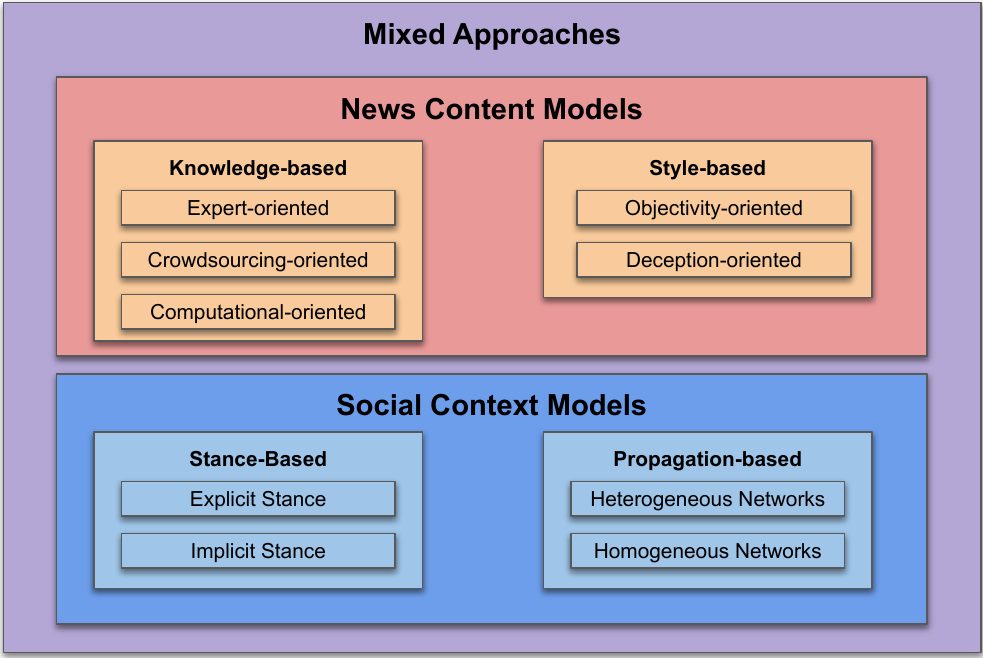
\includegraphics[scale=0.5]{FakeNewsDetectionModelsClassification}
    \caption[Characterization of Fake News Detection Models]{Characterization of Fake News Detection Models, Figure inspired by Figure 1 in~\cite{FakeNewsDetectionOnSocialMediaADataMiningPerspective_Shu}.}
    \label{fig:FakeNewsDetectionModelsClassification}
\end{figure}

\textbf{News Content Models.} Based on news content and fact-checking methodologies, these models are the starting point of fake news detection. News content models are classified as Knowledge-based and Style-based. We first introduce style-based models as they are the initial approaches for FND.
\begin{description}
    \item{\emph{Style-based}:} Previous research in psychology has mainly focused on style-based approaches to detect \emph{manipulators} in the text. Particularly deception detection techniques were popular and commonly developed in early works in criminology and psychology. We describe two different ways to approach style-based news content models, namely, \emph{Deception-oriented} and \emph{Objectivity-oriented}~\parencite{FakeNewsDetectionOnSocialMediaADataMiningPerspective_Shu}.
    \begin{itemize}
        \item \emph{Deception-oriented}: The initial approaches for automated fake news detection focus on news context and stem from deception detection in language. The first study that focuses deception detection in language~\parencite{DieEntwicklungDerGerichtspsychologischen_Undeutsch} hypothesized that the truthfulness of the statement is more important than the integrity of the reporting person, and there exist definable and descriptive criteria that form a crucial mechanism for the determination of the truthfulness of statements. Even though this study is from experimental psychology, it stresses the feasibility of defining a set of rules that determine the truthfulness of a statement.\\ An early study from criminology, Scientific Content Analysis (SCAN)~\parencite{SCAN_Sapir1987}, analyzes freely written statements.  In this process, SCAN claims to detect potential instances of deception in the text but cannot label a statement as a lie or truth. The next study for SCAN~\parencite{SCAN_Smith2001} is the first known study that correlates linguistic features with deceptive behavior using high-stakes data. Similar to SCAN, the subsequent studies  ~\parencite{CommunicationUnderStress_Adams, LyingWords_Newman} that link linguistic features to deception classify the owner of the statement as truth-teller or liar according to the frequency of deception indicators in the statement.\\Although for automated deception detection, defining a methodology is more challenging~\parencite{TheAccuracyConfidenceRelation_DePaulo}, early studies have shown that this task is achievable. A detailed study~\parencite{AutomatingLinguisticsBasedCues_Zhou} makes a structured approach using linguistic-based cues and draws attention to further studies for automating deception detection. In this study, the authors extend linguistic-based cues with complexity, expressivity, informality, and content diversity. Instead of using humans as cue identifiers, authors use \emph{Natural Language Processing} (NLP) techniques, namely an NLP tool called iSkim~\parencite{iSkim_Zhou}, to extract cues automatically. Another study also focuses on linguistic cue analysis. With a small dataset and employing the C4.5~\parencite{C45_Salzberg} algorithm, the authors reach 60.72\% accuracy using 15-fold cross-validation.\\Similarly, in ~\parencite{VerificatoinAndImplementationofLBDeceptionIndicators_Bachenko}, the authors developed a system for automatically identifying 275 truthful or deceitful statements with the use of verbal cues using Classification and Regression Tree (CART)~\parencite{ClassificationRegressioniTrees_Breiman}. Additionally, the studies ~\parencite{OnLyingAndBeingLiedTo_Hancock, OnDeceptionAndDeceptionDetection_Rubin} make use of a relatively small dataset and analyze linguistic-based cues. Rubin’s series of  studies~\parencite{OnDeceptionAndDeceptionDetection_Rubin, IdentificationOfTruth_Rubin, TruthAndDeception_Rubin, TowardsNewsVerification_Rubin} makes use of Rhetorical Structure Theory (RST) and Vector Space Modeling (VSM). The first captures the coherence of a story using functional relations among meaningful text units and delivers a hierarchical structure for each news story~\parencite{RST_William}. The second is the way to represent rhetorical relations in high-dimensional space. The authors utilized logistic regression as their classifier and reached 63\% accuracy.\\Furthermore, a study from Afroz and colleagues~\parencite{DetectingHoaxesFraudsAndDeception_Afroz} investigates stylistic deception and uses lexical, syntactic, and content-specific features. Lexical features include both character- and word-based features. Syntactic features represent sentence-level style and include frequency of function words from LIWC~\parencite{LIWC2007_Pennebaker}, punctuation, and POS tagging in which a text is assigned its morphosyntactic category~\parencite{POS_Daelemans}. Finally, content-specific features are keywords for a specific topic. For classification, the authors then leveraged Support Vector Machines (SVM)~\parencite{SVM_Hearst}. More comprehensive and modern approaches such as~\parencite{LiarLiarPantsOnFire_Wang} also leveraged the power of \emph{Convolutional Neural Networks} (CNN) to determine the veracity of news.
        \item \emph{Objectivity-oriented}: Objectivity-oriented news content models aim to detect indicators of the lessening of objectivity in news content~\parencite{FakeNewsDetectionOnSocialMediaADataMiningPerspective_Shu}. These indicators are observed in the news from misleading sources, such as hyperpartisan sources which display highly polarized opinions in favor of or against a particular political party. Consequently, this polarized behavior motivates the fabrication of news that supports the sources’ political views or undermines the opposing political party. \emph{Hyperpartisan news} are a subtle form of fake news and  defined as misleading coverage of events that did actually occur with a strong partisan bias~\parencite{FightingMisinformationOnSocialMedia_Pennycook}. Since the spread of hyperpartisan news can be detrimental, many approaches to detect hyperpartisanship in news articles have been developed. For instance, in~\parencite{AStylometricInquiry_Potthast}, the authors take a stylometric methodology to detect hyperpartisan news. In this study, the authors employ 10 readability scores, and dictionary features where each feature represent the frequency of words from a carefully crafted dictionary in a given document with the help of General Inquirer Dictionaries~\parencite{TheGeneralInquirer_Stone}. A competition for detecting hyperpartisan news~\parencite{SemEvalHyperpartisanNewsDetection_Kiesel} hosted several teams with a variety of ideas which include the utilization of n-grams, word embeddings, stylometry, sentiment analysis etc. The most popular method was the usage of embeddings, particularly the models that leveraged BERT~\parencite{BERT_Devlin}.\\ Also used for dissemination of hyperpartisan news~\parencite{SemEvalHyperpartisanNewsDetection_Kiesel}, another form of fake news that is evaluated under this focus is \emph{Yellow-journalism}, which utilizes clickbaits such as catchy headlines, images etc. that invokes strong emotions, and it aims to generate revenue~\parencite{ClickbaitDetectionUsingDL_Agrawal, ClickbaitAndTabloidStrategies_Dolors}. Studies that aim to detect clickbaits mainly focus on headlines. For example, in~\parencite{DivingDeepIntoClickbaits_Rony}, the authors construct a DNN in which they use distributed subword embeddings~\parencite{EnrichingWordVectorsWithSubwordInfo_Bojanowski, BagOfTricksForTextClassificatoin_Joulin} as features with an extension of skip-gram model~\parencite{DistributedRepresentationsOfWords_Mikolov}.
    \end{itemize}
    \item{\emph{Knowledge-based}}: Being the most direct way of detecting fake news, these approaches make use of external fact-checkers to verify the claims in news content~\parencite{FakeNewsDetectionOnSocialMediaADataMiningPerspective_Shu}. Fact-checkers are either sophisticated algorithms, domain experts or crowdsourced to assess the truthfulness of a claim in a specific context~\parencite{FactChecking_Vlachos}. With growing attention on fake news detection, automated fact-checking has drawn much attention, and considerable efforts have been made in this area~\parencite{AutomatedFactChecking_Thorne, OverviewOfCheckThat_Barroncede}. We categorize knowledge-based news content models as \emph{Expert-oriented}, \emph{Crowdsourcing-oriented}, and \emph{Computational-oriented}.
    \begin{itemize}
        \item \emph{Expert-oriented}: These approaches are essentially dependent on human domain experts who investigate the integrity of a
              news piece collecting relevant information and documents to come up with a decision about the truthfulness of a
              claim~\footnote{https://www.politifact.com/article/2018/feb/12/principles-truth-o-meter-politifacts-methodology-i/}. Platforms
              like Politifact~\footnote{https://www.politifact.com/} and EUfactcheck~\footnote{https://eufactcheck.eu/} are examples for expert-oriented fact-checking for all news from a variety of sources. These platforms label news in a range such that the label reflects the veracity of the news. A different approach for labeling is exercised by Snopes~\footnote{https://www.snopes.com/},
              which extends the same logic of Politifact by including different aspects of fact-checking such as Scam, Miscaptioned, Outdated, etc~\footnote{https://www.snopes.com/fact-check-ratings/}. Recently replaced by an irrelevant magazine website, another instance
              was Gossipcop~\footnote{https://web.archive.org/web/20190807002653/https://www.gossipcop.com/about/}, which dealt with celebrity fact-checking and contributed to the creation of fake news dataset~\parencite{FakeNewsNet_Shu}. Even though expert-based
              fact-checking is reliable, with the increasing magnitude of news stream and speed of spread, it is not scalable to fact-check every news piece by hand; thus, manual validation alone becomes insufficient~\parencite{ASurveyOnAutomatedFactChecking_Guo}.
        \item \emph{Crowdsourcing-oriented}: Powered by the wisdom of crowds~\parencite{WisdomOfCrowds_Galton}, crowdsourcing-oriented
              fact-checking is a collection of annotations that are afterward aggregated to obtain an overall result indicating the veracity of the
              news. Unlike professional fact-checkers, who are in short supply, this approach is scalable given that the crowd contains enough
              literate people~\parencite{ScalingUpFactChecking_Allen}.  For instance, Twitter launched a program called
              Birdwatch~\footnote{https://twitter.github.io/birdwatch/overview/}, in which the users are able to leave notes for tweets that they
              think contain misinformation. Furthermore, this tool allows users to rate each other’s notes, leading to the diversity of perspectives~\footnote{https://twitter.github.io/birdwatch/diversity-of-perspectives/}. Another example is from
              Facebook~\footnote{https://www.facebook.com/formedia/blog/third-party-fact-checking-how-it-works}, which uses a third party of
              crowdsourced fact-checkers called International Fact-Checking Network~\footnote{https://www.poynter.org/ifcn/} (IFCN).
        \item \emph{Computational-oriented}: Heavily dependent on external sources, computational-oriented models are scalable, automated
              systems that are designed to predict whether a claim is truthful or not. The studies that focused on this type of approach mainly try
              to solve two issues: (i) identifying check-worthy claims and (ii) estimating the integrity of claims~\parencite{FakeNewsDetectionOnSocialMediaADataMiningPerspective_Shu}.  The first issue requires the extraction of factual claims
              from news content or other related textual content. For example, in~\parencite{DetectingCheckWorthyClaims_Hassan}, the authors collect presidential debate transcripts, then label them into three classes with the help of crowdsourcing. Using annotated data and supervised learning techniques, the authors uncover some interesting patterns in these transcripts. Another study that covers both issues uses Wikipedia information to generate factual claims and then check whether a given claim is truthful or not~\parencite{FEVER_Thorne}.  The second issue, compared to the first one, requires the utilization of structured external sources. \emph{Open web} and structured \emph{knowledge graphs} are the two most prominent tools when tackling this issue. Open web tools analyze features like mutual information statistics~\parencite{UnsupervisedNamedEntityExtraction_Etzioni}, frequency, and web-based statistics~\parencite{WebBasedStatisticalFactChecking_Magdy}.  On the other hand, knowledge graphs are interconnected. One noteworthy example is ontologies such as DBPedia~\parencite{DBPedia_Auer}, using which one can define semantic relations and rules in order to infer whether a claim is correct~\parencite{SemanticFakeNewsDetection_Bracsoveanu}.
    \end{itemize}
\end{description}

\textbf{Social Context Models.} The interconnected design of social media can be leveraged by extracting user-based, post-based, and network-based features and utilizing these features to supplement news content models. Social context models exploit related user engagements for a news piece by capturing this external information from multiple angles. Two types of social context models are prominent: \emph{Stance-based} and \emph{Propagation-based}~\parencite{FakeNewsDetectionOnSocialMediaADataMiningPerspective_Shu}.
\begin{itemize}
    \item \emph{Stance-based}: Given a news piece, these approaches estimate the user’s stance toward a specific news topic. More
          formally, stance detection in social media deals with users’ viewpoints toward particular topics by means of various aspects related
          to users’ posts and characteristic traits~\parencite{StanceDetectionOnSocialMeda_Abeer}. The user’s stance information can be
          extracted either implicitly or explicitly. Implicit stance can be automatically obtained from social media posts with the help of NLP
          tools such as sentiment analysis~\parencite{StanceAndSentimentINTweets_Saif}. Explicit stances are rather easier to obtain since they
          are direct expressions of opinions or emotions. For example, “like” on Twitter or Facebook, “upvote” and “downvote” ratings on Reddit,
          and “like” and “dislike” on Youtube are explicit stances of users. A study that utilizes explicit stances called Some Like it
          Hoax, uses logistic regression and harmonic boolean label crowdsourcing for classification on a dataset they curated from Facebook.
          In the stance classification process, they consider the likes and the issuer of likes for each post. They state that logistic regression comes short in this task since it cannot learn anything about posts without likes~\parencite{SomeLikeItHoaxDataset_Tacchini}. An early example of implicit stance detection leverages the dialogic relations between authors
          by constructing graphs that represent the interaction between authors. They show that this information can improve the performance
          of stance-detection models~\parencite{StanceClassificationDialogicProps_Walker}. A more detailed
          study~\parencite{StanceClassificationOnTwitterDebates_Addawood} investigates stance classification considering lexical,
          syntactic, twitter-specific and argumentation feature types. Although some twitter-specific features can be considered as explicit stances, such as if the tweet is a retweet, if a tweet contains the title to an article, if a tweet contains a hashtag, etc., those
          features are later aggregated before it is fed to the classifier. The authors reach the highest F1 score using lexical and argumentation features. In literature, there are also implicit stance-based approaches that aim to detect the veracity of a news
          piece by exploring the relationship between a headline and the article~\parencite{ARetrospectiveAnalysisOfFNC_Hanselowski, StanceDetectionInFakeNews_Ghanem}.\\Another variation of stance-based detection is rumor detection. One example of a rumor detection model is a Bayes classifier that utilizes content-based, network-based, and twitter-specific meme features through \emph{Information Retrieval} (IR) techniques~\parencite{RumorHasIt_Qazvinian}.  In this study, the authors propose a general framework that leverages statistical models and maximizes a linear function of log-likelihood ratios to retrieve rumorous tweets. They show that the features they used contribute to their model's overall performance.
    \item  \emph{Propagation-based}: Inspired by the assumption that the veracity of a news event is highly correlated with the credibilities of related social media posts, propagation-based models employ the interrelations of related social media posts to classify a news piece as truthful or not~\parencite{FakeNewsDetectionOnSocialMediaADataMiningPerspective_Shu}. These models can be based on either \emph{homogeneous networks} or \emph{heterogeneous networks}.
          Homogeneous networks are built upon a single type of entity, such as a post or
          event~\parencite{NewsVerificationByExploitingConflictingSocialViewpoints_Jin}. A study
          by~\cite{NewsVerificationByExploitingConflictingSocialViewpoints_Jin} created homogeneous credibility networks for each topic which
          is extracted using an unbalanced version of the Joint Topic Viewpoint
          Model~\parencite{FindingAndArguingExpressions_Trabelsi}. These credibility networks consist of nodes as tweets and edges as links, defined by either supporting or opposing. On the other
          hand, heterogeneous networks can contain multiple types of entities such as events, sub-events, posts, comments, etc. For example, in~\parencite{NewsCredibilityEvaluationOnMicroblog_Jin}, the authors build a hierarchical propagation graph that contains events, sub-events, and messages from parent to child, respectively. Using an iterative method, they provide a globally optimal solution for the graph optimization problem in the study.\\Furthermore, an interesting study from a decade ago based its credibility estimation
          algorithm on PageRank and similarity scores. Their propagation network consists of graphs in which possible nodes are events, tweets that were posted about that event, and users who posted those tweets. A more recent study, which we also use in this thesis, is \emph{User Preference-Aware Fake News Dataset} (UPFD)~\parencite{UPFD_Dataset_Shu}. This dataset houses two different datasets, one from Politifact and one from Gossipcop. Its root nodes are news pieces, the child of the root node are the users who retweeted the news piece, and the children of the child node are the users who are assumed to have retweeted the news piece after its parent in terms of time. The authors use news content and social engagement information to construct the graph. The best-performing model is based on news and social context. It uses GraphSAGE~\parencite{GraphSAGE_Hamilton} as graph encoder and BERT~\parencite{BERT_Devlin} as the text encoder and reaches 84.62\% and 97.23\% accuracy on Politifact and Gossipcop, respectively.
\end{itemize}
We examined two types of FND models, namely,  news content and social context models. For each type, we further categorized then defined each type of model, and we gave examples for each. It is crucial to note that approaches are not necessarily purely news content or social context-based; they can be based on both news content and social context. For instance, like the example we gave in propagation-based social context models, GraphSAGE, there are models such as GNN-CL~\parencite{GraphNeuralNetworksWithContinualLearningFakeNewsDetection_Han} or
GCNFN~\parencite{FakeNewsDetectionUsingGeometricDeepLearning_Monti}, which are baseline models for UPFD~\parencite{UPFD_Dataset_Shu} and will be discussed in detail in the next section.\\
To summarize this section, we have introduced the history and definitions of fake news in subsection~\ref{subsec:fakeNewsDetection_fakeNews}. Then, we investigated the foundations of fake news and gave motivations for developing automated FND systems in subsection~\ref{subsec:fakeNewsDetection_FoundationsOfFakeNews}. Following that, we examined the evolution and characterized FND models in section~\ref{subsec:fakeNewsDetection_Evolution}. We have included at least two examples for each type of model and briefly summarized their approaches. We also briefly examined one of the datasets~\parencite{UPFD_Dataset_Shu} and models~\parencite{GraphSAGE_Hamilton} used in this thesis; however, in-depth information will be provided in the next chapter.\\
In~\ref{sec:explainableArtificialIntelligence}, we elaborate on the techniques available in explainable artificial intelligence. We discuss the qualities of a reasonable explanation, and we highlight the importance of the interpretability of a model. We give essential definitions that will be used throughout this thesis.

\section{Explainable Artificial Intelligence}
\label{sec:explainableArtificialIntelligence}
Understanding and interpreting a model's prediction is very important nowadays since this understanding allows to validate the reasoning of the model and extract rich information for a human expert, and can lead to increased trust in the model~\parencite{WhyShouldITrustYou_Riberio}. Furthermore, explanation of a model can help to improve the model~\parencite{AUnifiedApproach_Lundberg} and alleviate concerns raised by Ethical AI~\parencite{MachineBias_Angwin, EURegulationsOnDecisionMaking_Goodman}.
In this section, we introduce the background for XAI techniques that were used in this thesis. First, in~\ref{subsec:xai_foundations} we characterize XAI by following works from~\cite{TheMythosOfModelInterpretability_Lipton} and~\cite{XAIConceptsTaxonomies_Arrieta} and give definitions to clarify the taxonomy. Then, in~\ref{subsec:xai_aGoodExplanation}, we discuss the properties of good explanations, the goals of XAI and the evaluation techniques for explanation ethods. Finally, in~\ref{subsec:xai_overview} we briefly lay out the most frequently mentioned explanation methods in the literature, along with the ones we use in this thesis. We summarize each of them and cover explanation techniques offered to any kind of neural network.

\subsection{Foundations of Explainable Artificial Intelligence}
\label{subsec:xai_foundations}
Initial AI methods were not sophisticated enough to require additional explanation schemes. In the last years, expanding applications of DNNs have led to the adoption of these opaque systems even more. Although empirically successful thanks to enormous parameter spaces and numerous layers, DNNs are complex \emph{black-box} models in terms of  interpretability~\parencite{CanWeOpenTheBlackBoxOfAI_Castelvecchi}.\\
In the XAI context, \emph{black-box} or \emph{opaque} models are considered to be the opposite of \emph{transparent} because they require a further search to understand their inner workings~\parencite{TheMythosOfModelInterpretability_Lipton}. Accordingly, humans hesitate to use
systems that are not directly interpretable and reliable~\parencite{xAIForDesigners_Zhu}, making \emph{interpretability} essential. Moreover, from a legal perspective, the notion \emph{right to explanation} brings more attention to interpretabilty~\parencite{TheMythosOfModelInterpretability_Lipton}. Particularly in situations such as when:
\begin{itemize}
    \item The prediction of AI directly affects human life, e.g., fully autonomous cars in traffic, medical AI assistants etc.
    \item The reasons behind an AI system’s decision can not be clearly determined.
\end{itemize}
With the additional demand from the Ethical AI field~\parencite{EURegulationsOnDecisionMaking_Goodman}, the research community has put in a great amount of effort to gap the bridge between a black-box model and its interpretability. However, the lack of consensus on taxonomy has led to synonymous usages of interpretability. The early definitions for interpretability were too broad, describing it as essentially an additional design driver when building a model~\parencite{TheBayesianCaseModel_Kim} or a requirement for \emph{trust}~\parencite{InteractiveAndInterpretableMLModels_Kim}. But can trust be defined in an objective way? Is the accuracy or F1 score of the model is enough to trust a model? To answer the first question, \cite{TheMythosOfModelInterpretability_Lipton} argues that trust is subjective and it is not technically defined. To answer the second question, taking only the performance metrics as a baseline for trust in the model is shown to be an incorrect approach, particularly studies that analyze models with \emph{adversarial examples}~\parencite{DetectingAdversarilaImageExamples_Bin, AdversarialExamples_Yuan}. Moreover, ~\cite{TowardsARigorousScienceML_Velez} argues that the need for interpretability comes from the \emph{incompleteness} of the problem formalization.\\
Instead of trying to find a technical definition for interpretability, we can categorize existing systems in terms of their transparency.
\cite{TheMythosOfModelInterpretability_Lipton} states two properties for interpretable models: \emph{transparency} and \emph{post-hoc interpretability}. The definition for the first and its related terms are given as in the following,
\begin{definition}[\emph{Understandability}]
    “\emph{Denotes the characteristic of a model to make a human understand its function - how the model works - without any need for explaining its internal structure or the algorithmic means by which the model processes data internally}”~\parencite{MethodsForInterpretingAndUnderstandingDNNs_Montavon,XAIConceptsTaxonomies_Arrieta}.
\end{definition}
\begin{definition}[\emph{Transparency}]
    “\emph{A model is considered to be transparent if by itself it is understandable}”~\parencite{XAIConceptsTaxonomies_Arrieta}.
\end{definition}
To elaborate further, we discuss degrees of transparent models as not all models provide the same extent of understandability~\parencite{XAIConceptsTaxonomies_Arrieta}. Both in~\cite{TheMythosOfModelInterpretability_Lipton} and \cite{XAIConceptsTaxonomies_Arrieta} the
categorization is made as: \emph{simulability}, \emph{decomposability}, and \emph{algorithmic transparency}. We discuss each of them briefly.
\begin{itemize}
    \item \emph{Simulability}: Denotes the model’s characteristic to be simulated or thought only by a human. Thus, the complexity of a model
          plays an important role here. Models that can be presented to a human in terms of text and visualizations are considered
          interpretable~\parencite{WhyShouldITrustYou_Riberio}, and in this case, models this elementary fall into simulatable models
          category~\parencite{XAIConceptsTaxonomies_Arrieta, RegressionShrinkage_Tibshirani}.
    \item \emph{Decomposability}: Represents the model’s characteristic to explain each part of the model. Basically, when all components of a model
          are simulable, then that model is decomposable~\parencite{TheMythosOfModelInterpretability_Lipton} given that the inputs are already interpretable~\parencite{XAIConceptsTaxonomies_Arrieta}.
    \item \emph{Algorithmic Transparency}: Deals with the user’s comprehension of the input’s journey from entering the model to becoming a prediction~\parencite{TheMythosOfModelInterpretability_Lipton, XAIConceptsTaxonomies_Arrieta}. For example, linear models can be considered algorihtmically transparent since the user can understand how the model can act in a given situation~\parencite{AnIntroductionToStatisticalLearning_Gareth}.
\end{itemize}
The second property of interpretable models, \emph{post-hoc explainability}, aims to improve the interpretability of not readily interpretable models. It does so by means of \emph{text explanations}, \emph{visual explanations}, \emph{local explanations}, \emph{explanations by example},
\emph{explanations by simplification}, and \emph{feature relevance explanations} techniques~\parencite{TheMythosOfModelInterpretability_Lipton, XAIConceptsTaxonomies_Arrieta}. In a more general sense, post-hoc explainability methods can be grouped into three categories in terms of the knowledge of the target model, granularity of focus, and form: \emph{model-specific or model-agnostic}, \emph{local or global} and \emph{form}. The first category refers to the explainability method's assumption on the model's structure. \emph{Model-specific} techniques can be utilized with a limited set of models since these techniques make an assumption on the model to be explained. On the other hand, \emph{model-agnostic} techniques are designed in such a way that does not require knowledge about model's inner workings~\parencite{XAIConceptsTaxonomies_Arrieta,ASurveyOfMethodsForExplainingBlackBoxModels_Guidotti}. The second category denotes the explanation's domain. \emph{Local} explanations reason about a particular prediction of a model at feature level~\parencite{TowardsARigorousScienceML_Velez} (e.g. compute a saliency map by taking the gradient of the output with respect to a given input vector~\parencite{TheMythosOfModelInterpretability_Lipton}), whereas global explanations aim to outline the model's general behavior on the dataset~\parencite{XAIConceptsTaxonomies_Arrieta, ASurveyOfMethodsForExplainingBlackBoxModels_Guidotti,TowardsARigorousScienceML_Velez}. Global explanations are usually presented in the structure of a series of rules~\parencite{InterpretableDecisionSets_Lakkaraju}. The third and last category, form of the explanation is the manner that is conveyed to the user. We will discuss specific forms of explanation in detail after we give a definition of \emph{explainability}, since from now on we talk about the explainability of a model rather than its interpretability.
\begin{definition}[Explainability]
    “\emph{Explainability is associated with the notion of explanation as an interface between humans and a decision maker that is, at the same time, both an accurate proxy of the decision maker and comprehensible to humans.}”~\parencite{XAIConceptsTaxonomies_Arrieta, ASurveyOfMethodsForExplainingBlackBoxModels_Guidotti}
\end{definition}
\begin{itemize}
    \item \emph{Text explanations} are techniques that learn to produce textual expressions that assist user to understand the outcomes of the model~\parencite{TowardsExplainableNeuralSymbolic_Bennetot}.
    \item \emph{Visual explanations} are techniques that supplement a model's explainability by visualizing the model's behavior. Due to the mismatch between high-dimensional nature of  complex ML systems and the capacity of human reasoning~\parencite{HowTheMachineThinks_Burrell}, visual explanations often employ dimensionality reduction practices~\parencite{XAIConceptsTaxonomies_Arrieta}.
\end{itemize}
From the perspective of explainability, one would intuitively prefer transparency since transparent models
can be explained with ease. However, some works argue that as transparency of a model increases their performance usually tends to decrease~\parencite{ExplaniableAIASurvey_Dosilovic}, although other works argue that this is not necessarily true, particularly in cases where the data is well structured and the quailty and value of available features is outstanding~\parencite{StopExplainingBlackBoxmodels_Rudin}. Furthermore, considering FND models, the
need for big and complex models can not be avoided since news pieces tend to be long texts, or social networks are represented as graphs, thus forcing SOTA FND models to utilize complex approaches that decreases transparecy such as word embeddings, data fusion, graph data structure~\parencite{UPFD_Dataset_Shu}.\\
On the other hand, although global explanations can be helpful to domain experts by providing information about what model has learnt on a global level, it might be difficult to obtain~\parencite{TheMythosOfModelInterpretability_Lipton}. Instead, local explanation methods are more easier to obtain and more practical for real-world applications. For example, if a user requests an explanation for a prediction, local explanations can provide it, which also complies with "right to explanation"~\parencite{EURegulationsOnDecisionMaking_Goodman}.\\
Depending on the model adopted for FND, we might be required to use model-specific or model-agnostic approaches. For instance, when dealing with a GNN, model-agnostic approaches do not provide easily interpretable explanations, thus requiring a model-specific explanation method. On the other hand, when dealing with a DNN model-agnostic post-hoc approaches are usually the choice~\parencite{XAIConceptsTaxonomies_Arrieta}. Therefore, for FND models used in this thesis, we are required to adopt both model-agnostic and model-specific post-hoc approaches. Below we list types of post-hoc approach as listen in~\parencite{XAIConceptsTaxonomies_Arrieta}.
\begin{itemize}
    \item \emph{Explanations by example}, a method suggested by~\cite{CaseBasedExplanation_Caruana}, focus on obtaining representative information from a model by providing explanations for an example that sufficiently illustrates the inner workings of the model~\parencite{HowToExplainIndividualClassificationDecisions_Baehrens, XAIConceptsTaxonomies_Arrieta}.
    \item \emph{Explanations by simplification} techniques construct a new and simplified system to provide explanations for a model. These simplified systems keep the performance of the original model while displaying less complexity~\parencite{XAIConceptsTaxonomies_Arrieta}.
    \item \emph{Feature relevance explanations} compute feature relevance scores for a model's variables in order to determine the effect of a feature has upon a model~\parencite{XAIConceptsTaxonomies_Arrieta}.
\end{itemize}
We discussed what kind of explanation methods we can adopt and how these methods can shape the design of a model and the forms of explanations that aims to convey information about the model's behavior. It is possible to see a combination of the previously mentioned explanation forms. In order to present the user with an comprehensible explanation, we characterize a good explanation and define its important properties in the next subsection.

\subsection{What Makes A Good Explanation}
\label{subsec:xai_aGoodExplanation}
In literature, the requirements for a \emph{good explanation} are rigorously researched. However, there is not a clear definition of how an explanation should look like or convey to the user. It is challenging to objectively define what makes a good explanation~\parencite{XAIConceptsTaxonomies_Arrieta}. In order to tackle the issue of subjectivity of explanations, XAI draws wisdom from social and cognitive sciences. A comprehensive study on social sciences and XAI by~\cite{ExplanationInAI_Miller}, analyzes explanations in terms of the content, the explainer and the explainee. The author argues that the research in AI is lacking knowledge about the properties and structure of an explanation.  The major findings on how a good explanation should be are outlined below.
\begin{itemize}
    \item Explanations are \emph{contrastive}~\parencite{ContrastiveExplanation_Lipton, XAI_BewareInmatesRunningTheAsylum_Miller}. When presented with counterfactual explanations, users can understand the decision made by the model easier~\parencite{ExplainableAndInterpretableModels_Escalante, MLCVPatternRecognition_Lopez, MLCVPatternRecognition_Lopez, CounterfactualsInXAI_Byrne}. For example, rather than asking why event $A$ occurred, we ask why event $A$ occurred instead of an event $B$~\parencite{ExplanationInAI_Miller,XAIConceptsTaxonomies_Arrieta}.
    \item Explanations are \emph{selective}. Presenting all the causes for an event to a human is pointless, since humans are inclined to select a couple main causes out of numerous, sometimes countless, causes as shown in~\parencite{ExplainingCollaborativeFiltering_Herlocker}. Accordingly,~\cite{ExplanationInAI_Miller} argues that this selection process is shaped by specific cognitive biases.
    \item Explanations are \emph{social}. They are conveyed from explainer to explainee via a social interaction. Hence, explanations are transferred through the frame of explainer's beliefs about the explainee's beliefs~\parencite{ExplanationInAI_Miller}.
    \item Probabilities probably don't matter. Even though probabilities matter when creating the explanations, the usage of these statistical relations in explanations is not as effective as that of causes. If the underlying causal explanation is not included, then the utilization of statistical generalisations is not sufficient~\parencite{ExplanationInAI_Miller}.
\end{itemize}
It should be noted that the characteristics of a good explanation is not limited to the ones mentioned above. These are the most prominent characteristics of numerous which is discussed in~\parencite{ExplanationInAI_Miller} detail. An important aspect here is that the explanations are provided to an \emph{explainee} who is the \emph{audience} in~\parencite{XAIConceptsTaxonomies_Arrieta}, which refers to the person receving the explanation. It is further noted in~\parencite{XAIConceptsTaxonomies_Arrieta} that explanations are dependent on the audience, i.e., an explanation meant for an end-user will not be enough for a domain expert or an explanation for a domain expert might be too complicated for an end-user. Also, we will refer to the expainee as \emph{audience} from now on.\\
Main target audience is the main driver when considering the needed outcomes for an explanation.~\cite{XAIConceptsTaxonomies_Arrieta} summarizes the pursued goals when trying to attain explainability. These are listed below.
\begin{itemize}
    \item \emph{Trustworthiness} deals with the assurance of a model's intended behavior when the model is presented with real-world scenarios~\parencite{TheMythosOfModelInterpretability_Lipton, StructuringDimensionsForCollaborative_Antunes}. Some studies highlight the importance of \emph{trustworthiness} as a requirement for explainability~\parencite{WhyShouldITrustYou_Riberio, InteractiveBayesianCaseModel_Kim}. The main target audience for this goal is domain experts, and users affected by the model decisions~\parencite{XAIConceptsTaxonomies_Arrieta}.
    \item \emph{Confidence} refers to the robustness and stability of a model~\parencite{XAIConceptsTaxonomies_Arrieta}.~\cite{Stability_Yu} argues that stability is a prerequisite when obtaining explanations from a model. Moreover,~\parencite{XAIConceptsTaxonomies_Arrieta} argues that trustworthy explanations should not be obtained from unstable models. The audience relevant for this goal are domain expers, developers, managers, and regulatory entities.
    \item \emph{Fairness} refers to a model's potential to ensure a fair prediction for a user affected by the model's prediction on the basis of characteristics such as age, race, gender, etc~\parencite{XAIConceptsTaxonomies_Arrieta, FairnessInML_Oneto}. The audience for this goal consists of users affected by model decisions and regulatory entities.
    \item \emph{Transferability} refers to the model's capability to perform on unseen data. It is a desired goal to have not just for explainability but also for obtaining a good performance from the model~\parencite{AppliedPredictiveModeling_Kuhn}. The audience for this goal is domain experts and data scientists.
    \item \emph{Causality} denotes the causal relationships between variables of a model~\parencite{Causality_Pearl}. It aims to provide causal information among the data variables. Its main audience is domain experts, managers, and regulatory entities~\parencite{XAIConceptsTaxonomies_Arrieta}.
    \item \emph{Informativeness} is a goal meant for all users and it deals with the information provided by the model. In order to fill the gap between user's decision and the prediction of a model, a massive amount of information about the problem at hand needs to be conveyed to the end user~\parencite{XAIConceptsTaxonomies_Arrieta}.
    \item \emph{Accessibility} refers to the possibility of end users getting more involved in a model's development or improvement~\parencite{XAI_BewareInmatesRunningTheAsylum_Miller}. The audience for this goal includes product owners, managers, and user affected by model decisions.
    \item \emph{Interactivity} denotes a model's capability to interact with the user~\parencite{InteractiveAndInterpretableMLModels_Kim}. The main audience consists of domain experts and users affected model decisions.
    \item \emph{Privacy awareness} is a goal not frequently seen in the literature. It deals with the learnings of a model's internal representation such that these learnings might pose a privacy breach. From the opposite perspective, it is a differential privacy breach when an unauthorized third party can explain the inner workings if a trained model~\parencite{XAIConceptsTaxonomies_Arrieta}.
\end{itemize}
On the other hand, for a given explanation and its preferred characteristics, how do we objectively evaluate an explanation? For example, considering a model, the evaluation metrics obtained from the test set reflect the model's overall performance on unseen data and allow to compare different models that use the same dataset~\parencite{PMLB_Olson}. For example, metrics like accuracy, F1 score, recall, and precision are often used in the evaluation of models. Given that there are numerous metrics, it should be noted that different domains and models may require different evaluation metrics~\parencite{BeingAccurateIsNotEnough_McNee, AReviewOnEvaluationMetrics_Hossin, PeeringIntoTheBlackBoxOfAI_Handelman}. For a comprehensive study on the evaluation metrics of ML models, please refer to~\parencite{EvaluatingLearningAlgorithms_Japkowicz}.
Similar to models, explanations require evaluation methods that can quantify their performance. So far, we have seen that explanations might have different audiences, they can take several forms, and they have desired properties. Therefore, like models, there should be a set of explanation evaluation methods which focus on different categories of explanation approaches. In fact, a rigorous study by~\cite{TowardsARigorousScienceML_Velez} lays out the categorization of explanation evalution approaches. The authors split the evaluation methodologies into three:
\begin{enumerate}
    \item \emph{Application-grounded evaluations} involve conducting experiments on real humans who are domain experts interacting with explanations in a real-world application. This kind of evaluation directly tests the objective of the system, thus, attaining high performance with respect to application-grounded evaluation suggests good evidence of the explanation's success. The fact that we need humans interacting with a real-world application in an environment which can be observed for experimentation makes this type of evaluation more specific and thus the most costly of all three types of evaluation~\parencite{TowardsARigorousScienceML_Velez}.
    \item \emph{Human-grounded evaluations} are constructed by simpler experiments conducted on real humans who are not necessarily domain experts. Although this type of evaluation is less specific compared to the application-grounded evaluations, it offers more flexibilty and less costly. It is a good choice when the task is to test the quality of an explanation in a general sense~\parencite{TowardsARigorousScienceML_Velez}. For example, a recent study~\parencite{AHumanGroundedEvaluationBenchmark_Mohseni} used human attention maps that overlay on images as explanations and asked users to rate the decision made by the model. The study further argues that the evaluation on these attention maps can be utilized to understand the \emph{trustworthiness} of a model.
    \item \emph{Functional-grounded evaluations} do not include real humans, instead this kind of evaluations use a formal definition of interpretability as a proxy to assess the explanation's quailty. The lack of human dependency makes them favorable due to the low cost. Typically, these evaluations are preferred when conducting experiments with humans in the loop might be unethical. The challenge with these evaluations is to select the right proxy models. Accordingly, when possible, it is considered good practice to first obtain proxies that were verified, for instance, by human-grounded evaluations~\parencite{TowardsARigorousScienceML_Velez}.
\end{enumerate}
From high cost to low cost, and more specific to more broad, one can opt for an evaluation technique to obtain a performance indicator of an explanation. As discussed above, each approach require a completely different setting, which brings their shortcomings with it. For instance, depending of the availability of resources such as time, finances, expertise of the user or sufficiency of human subjects one might have to opt for a different evaluation technique.\\
Having highlighted important characteristics of a good explanation, we now move forward to the frequently mentioned techniques used in XAI. We mostly focus on post-hoc local explanation techniques and outline their contribution to this thesis.

\subsection{Overview of Techniques in Explainable Artificial Intelligence}
\label{subsec:xai_overview}
As discussed in the last section, when contructing an explanation method, one has to consider the audience,
opt between model-specific or model-agnostic, local or global explanations, and also, utilize various forms
of explanation. In literature, there exist various combinations of previously mentioned options. For transparent models, no further explanation method needed, one can obtain relevant information in
the forms of weights or attention scores, given that the features are simple enough~\parencite{XAIConceptsTaxonomies_Arrieta}. In particular, we talk about explanation methods that were frequently mentioned
in studies and relevant for this thesis.\\
First, we discuss the initial methodologies aimed to gain insight from a black-box model. The one of the initial approaches was to ask the question: \emph{What happens if we remove this part of the input?} \emph{Sensitivity Analysis} (SA) deals with analytical assessment of the effect of an omitted input variable on the uncertainty of a model~\parencite{SensitivityAndGeneralizationInNNs_Novak}. SA can be done on two levels, local and global. \emph{Local Sensivity Analysis} (LSA) assesses the impact of the changes in the input on the output whereas \emph{Global Sensitivity Analysis} (GSA) examines the effect of each variable (feature) with respect to the variations of all parameters~\parencite{InputPerturbationSensitivity_Rao}. In literature, there are a variety of approaches for both GSA and LSA. For instance,~\cite{SensitivityAndGeneralizationInNNs_Novak} constructs a GSA that employs the partial derivative of each parameter in the back-propagation algorithm to explore the change rule, which admits the \emph{Input-Perturbation-Sensitivity} (IPS) that allows to obtain global sensitivity. An interesting example of a GSA and LSA fusion approach,~\cite{SensitivityAnalysisForPNNs_Kowalski}, utilizes LSA to reduce the number of input features and GSA to reduce the number of patterns learned by a model.\\
Another approach was to calculate relevance scores for each feature using saliency maps. The usage of saliency maps first appeared in CNNs for images~\parencite{DeepInsideCNNs_Simonyan}, then extended to NLP in~\cite{AskTheGRU_Trapit, ExtractionOfSalientSentences_Denil}. Typically, salience maps compute a gradient to get a relevance score to an input feature. In other words, they convey information about the model's sensitivity with respect to the input.\\
A popular method used in XAI is \emph{Layer-wise Relevance Rropagation} (LRP) which was first introduced for \emph{Fully Connected Networks} (FCNs) and CNNs in~\cite{LRP_Lapuschkin}, then extended to \emph{Recurrent Neural Networks} (RNNs) in~\cite{ExplainingRNNs_Arras}. LRP assumes that a model can be \emph{decomposed} into several layers which can contain feature relevant information. From the last layer to the input layer, LRP computes a relevance score for each dimension of the vector at a layer, and as LRP moves backwards in the layers, the sum of relevance scores do not change, staying always equal to the prediction probability~\parencite{LRP_Lapuschkin}.\\
Similar to LRP, a study for explaining DNNs offers another solution named \emph{Deep Learning Important FeaTures} (DeepLIFT)~\parencite{DeepLIFT_Shrikumar}. This approach addresses two shortcomings of LRP, namely, the failure to model saturation caused by activation functions, and the possibility of getting misleading importance scores due to discontinuous gradients. Combining techniques from LRP and integrated gradients~\parencite{GradientsOfCounterfactuals_Sundararajan}, DeepLIFT computes importance scores based on the \emph{difference-from-reference} approach which allows propagation of information even if the gradient is zero. Difference-from-reference is a method which involves determining a reference then getting the difference between the reference and the output. This method is also later adopted by to create DeepSHAP~\parencite{AUnifiedApproach_Lundberg}.\\
In contrast to model-specific approaches like LRP and DeepLIFT, \emph{Locally Interpretable Model-agnostic Explanations} (LIME), as the name suggests, is a model-agnostic method. LIME interprets the predictions of any black-box model by approximating the model around a prediction. This approximation allows to obtain a locally faithful and interpretable version of the model~\parencite{WhyShouldITrustYou_Riberio}.\\
So far, there is no study that unifies all the works to create one explainability framework. To address this lack of unification,~\cite{AUnifiedApproach_Lundberg} offers \emph{SHapley Additive exPlanation} (SHAP) framework, in which the authors utilize recent studies from game theory based on~\parencite{GameTheory_Shapley}. These studies are \emph{Shapley regression values}~\parencite{AnalysisOfRegressionInGameTheory_Lipovetsky}, \emph{Shapley sampling values}~\parencite{ExplainingPredictionModels_Strumbelj}\emph{Quantitative input influence}~\parencite{AlgorithmicTransparencyViaQuantitativeInputInfluence_Datta}, and recent approaches like LIME, DeepLIFT are utilized to create a model-agnostic and model-specific explainers. SHAP values measure the feature importance and obtained via Shapley values of conditional expectation function of a model~\parencite{AUnifiedApproach_Lundberg}. Model-agnostic SHAP values are computed using Shapley sampling values method which uses an approximation of a permutation adaption of of classic Shapley value estimation. For example, \emph{KernelSHAP} employs LIME with linear explanations and Shapley values to find a weighting kernel that enables regression based estimation of SHAP values. On the other hand, the authors propose \emph{LinearSHAP} which can approximate Shapley values using weights for linear models, and \emph{DeepSHAP} which connects DeepLIFT with Shapley values, \emph{Low-order SHAP}, and \emph{Max SHAP} for model-specific explainers. We will discuss SHAP values further in Chapter~\ref{chapter:explainability_of_fnd_models}.\\
In literature, there is a lack of explanation methods for GNNs. GNNs require graphs as input and an output for either graph or node depending on the focus of the task~\parencite{DeepLearningOnGraphs_Zhang}. Graphs are capable of representing rich relational information between nodes and the node feature
information~\parencite{DeepLearningOnGraphs_Zhang, GNNsAReview_Zhou}. GNNs are powerful tools that are able to learn relational information between nodes as well as node features, making them a perfect candidate for analyzing social media networks~\parencite{BeyondSigmoids_Zang}. In our case, we want to understand how a GNN behaves when classifying fake and real news pieces and their propagation networks. A study by~\cite{GNNExplainer_Ying} proposes a model-agnostic approach called \emph{GNNExplainer} to explain predictions made by GNNs. \emph{GNNExplainer} takes a trained GNN, input graph(s) and its prediction(s) ad it returns explanations in the form of subgraph(s) of input
graph(s) along with the most influential node feaures for the prediction. These subgraphs are constructed by maximizing the mutual information between the subgraph and the input graph with respect to the
prediction~\parencite{GNNExplainer_Ying}.\\
Bearing in mind the FND models and explanation methods discussed one can use LIME, DeepLIFT, or SHAP for news content models which are essentially DNNs with textual data as inputs. Especially for understanding which words or word groups are of the most importance, SHAP provides text plots and easily interpretable importance scores. Therefore, when assessing our choice of news content model, we employ SHAP framework, in particular, DeepSHAP. On the other hand, for GNNs the choice is straightforward as there is only one choice. Although, GNNExplainer can be helpful to identify the most important spreaders of a news piece which will be discussed in Chapter~\ref{chapter:explainability_of_fnd_models}.\\
To conclude this chapter, it should be noted that due to the numerous studies in the literature, we did not cover all explanation methods, but an extensive study can be found in~\parencite{InterpretableMachineLearning_Molnar}. Moreover, we were not able to fully cover the psychological and social background of explanations as we did for fake news, however~\cite{ExplanationInAI_Miller} provides a rigorous research in that field. In the next chapter, we elaborate on FND models that were used in this thesis. We show how a neural network produces a prediction for a given input. We share our analysis on both textual and graph datasets. After talking about model parameters and hyperparameters, we evaluate our models and talk about the evaluation process. Also, we examine issues like early fake news detection and model aging, particularly for our SOTA FND models.
